\ChapterImageStar[cap:benchmarking]{Benchmarking}{./images/fondo.png}\label{cap:benchmarking}

\mbox{}\\
\section{Definición de las pruebas}

Para evaluar el rendimiento de distintas tecnologías de contenerización —específicamente Docker, Podman, LXC, LXD y Containerd— se diseñó un conjunto de pruebas orientadas a medir aspectos clave del desempeño en entornos controlados. Las pruebas incluyeron el consumo de CPU y memoria RAM, el tiempo de arranque de los contenedores, el \textit{throughput} de red y la latencia de acceso a disco. 

Para garantizar la repetibilidad y objetividad de los resultados, se desarrollaron scripts en \textit{Bash} que automatizan la ejecución de cada métrica en condiciones homogéneas. Estas pruebas permiten comparar las tecnologías evaluadas bajo criterios cuantificables y facilitar un análisis técnico de sus capacidades en escenarios reales de uso.

\section{Construcción de las pruebas}

La construcción de las pruebas se llevó a cabo mediante el desarrollo de scripts automatizados en \textit{Bash}, diseñados para ejecutarse de forma uniforme sobre cada tecnología de contenerización evaluada. Cada script fue responsable de iniciar contenedores, ejecutar cargas de trabajo específicas y recolectar métricas de rendimiento relevantes.

Para medir el consumo de CPU y memoria RAM, se utilizó \texttt{pidstat}, una utilidad que permite la medición del consumo de recursos. El tiempo de arranque se determinó midiendo el intervalo entre la orden de inicio del contenedor y el momento en que estuvo completamente operativo. 

Para evaluar el \textit{throughput} de red se emplearon herramientas como \texttt{iperf}, mientras que la latencia de disco fue medida utilizando \texttt{fio}. Todas las pruebas fueron ejecutadas múltiples veces para reducir el impacto de variaciones puntuales y asegurar la confiabilidad de los resultados. Los scripts fueron programados para ejecutarse 10 veces; al final se extrae un promedio y este constituye el puntaje final de la tecnología de contenerización en cuestión.

En el repositorio \underline{\href{https://github.com/Anubis-1001/benchmark-tecnologias-de-contenerizacion} {\texttt{ GitHub benchmarking}}} se pueden encontrar los scripts resultantes de este proceso.

\section{Resultados de las pruebas}

Los resultados obtenidos a partir de las pruebas evidencian diferencias significativas en el rendimiento entre las tecnologías de contenerización evaluadas. Estos se pueden consultar en el archivo de Excel \underline{\href{https://docs.google.com/spreadsheets/d/1Ce37Sm3Swyfa88Ur1yQbLarq_D86obUIAGGJocgQbUE/edit?usp=sharing} {\texttt{benchmarking\_tecnologias}}}.

En términos de consumo de CPU, Docker y Containerd presentan las mejores métricas; en consumo de memoria RAM, LXC y LXD mostraron un mejor uso de los recursos. En cuanto al tiempo de arranque, Containerd destacó por su velocidad, seguido de cerca por Docker, mientras que LXC presentó un arranque considerablemente más lento en comparación con las demás tecnologías.

Para el \textit{throughput} de red, todas las tecnologías mostraron un desempeño comparable, siendo LXC el más destacado; no obstante, Podman quedó muy por debajo en esta métrica. Finalmente, en la medición de latencia de disco, LXD y Containerd obtuvieron los mejores resultados, lo que sugiere una gestión de E/S más directa y liviana.

Estos resultados permiten establecer un panorama claro de fortalezas y debilidades de cada solución, según el tipo de carga o entorno de ejecución esperado.

\section{Métricas de rendimiento}

De la ejecución de las pruebas se obtuvieron las siguientes métricas de rendimiento:

\begin{figure}[H]
    \centering
    \includegraphics[scale=0.5] {tablas-images/cp4/cpu.png}
    \caption{Métricas de uso de CPU}\label{fig:tabla-metricas-cpu}
\end{figure}
\begin{figure}[H]
    \centering
    \includegraphics[width=\textwidth] {tablas-images/cp4/ram.png}
    \caption{Métricas de uso de RAM}\label{fig:tabla-metricas-ram}
\end{figure}
\begin{figure}[H]
    \centering
    \includegraphics[width=\textwidth] {tablas-images/cp4/io.png}
    \caption{Métricas de entrada/salida}\label{fig:tabla-metricas-io}
\end{figure}
\begin{figure}[H]
    \centering
    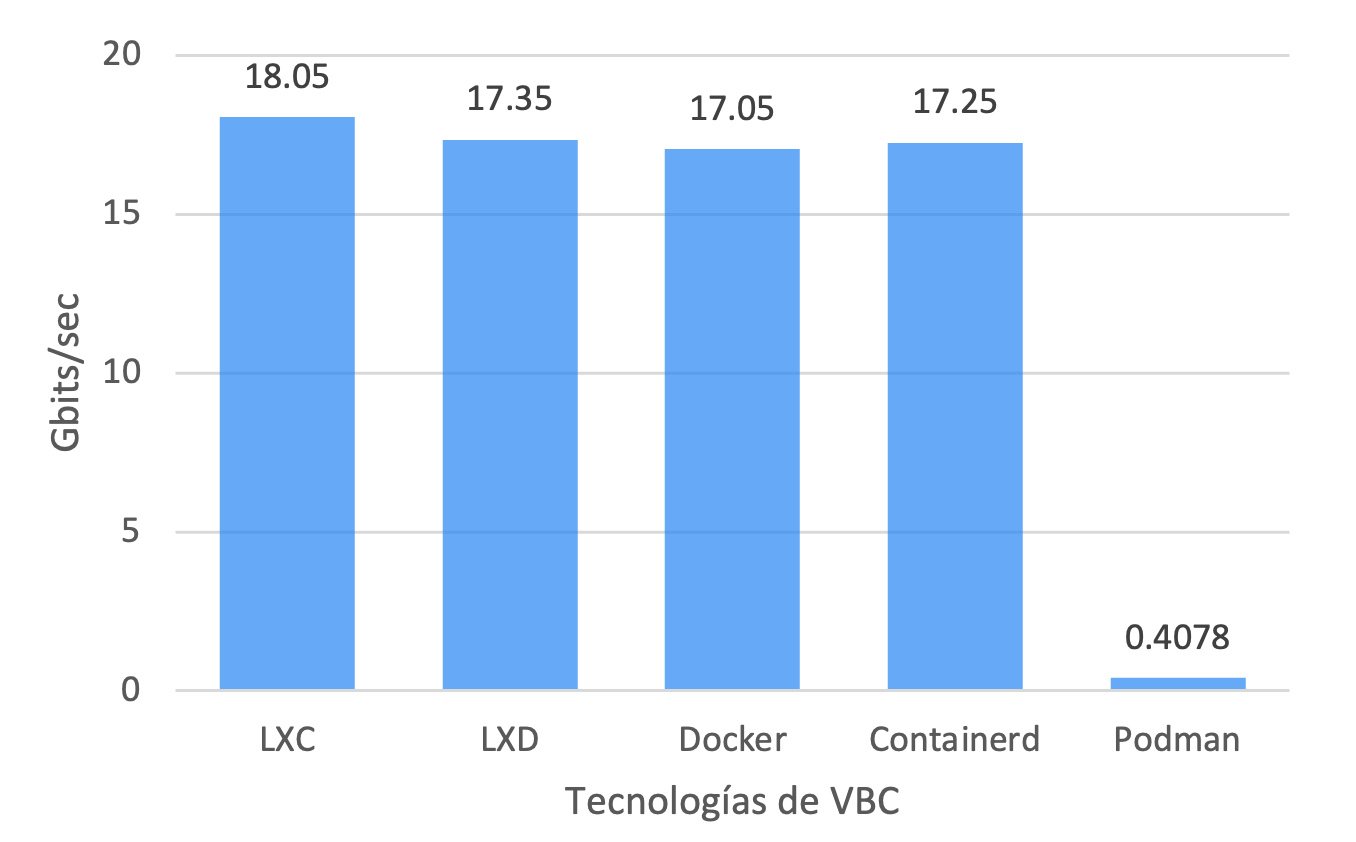
\includegraphics[width=\textwidth] {tablas-images/cp4/THROUGHTPUT.png}
    \caption{Métricas de throughput}\label{fig:tabla-metricas-throughput}
\end{figure}

\section{Análisis de los resultados}

Los resultados obtenidos a partir de las pruebas permiten identificar comportamientos diferenciados entre las tecnologías de contenerización evaluadas. \textbf{Containerd} se posiciona como una de las soluciones más equilibradas, con excelente tiempo de arranque, bajo uso de CPU y buena latencia de disco, lo que lo hace ideal para entornos donde la eficiencia es prioritaria.

\textbf{LXC} mostró consistentemente el menor consumo de recursos y alto rendimiento en red, lo que lo convierte en una opción sólida para sistemas embebidos o despliegues que requieren un uso mínimo de \textit{overhead}. 

Por otro lado, \textbf{Docker} ofreció un rendimiento aceptable, pero con mayores niveles de consumo de CPU y latencia de disco, compensados por su madurez y ecosistema. 

\textbf{LXD}, al estar basado en LXC, heredó parte de sus beneficios, especialmente en uso de red, aunque con un ligero incremento en el tiempo de arranque. 

En contraste, \textbf{Podman}, si bien eficiente en uso de CPU y memoria, presentó resultados considerablemente bajos en el \textit{throughput} de red y alta latencia de disco, lo cual podría limitar su aplicación en cargas sensibles a E/S o comunicación intensiva.

\vspace{0.5em}

\noindent En resumen, la elección de la tecnología de contenerización debe considerar el caso de uso específico: \textbf{Containerd} y \textbf{LXC} sobresalen en eficiencia general; \textbf{Docker} y \textbf{LXD} ofrecen robustez y facilidad de integración; mientras que \textbf{Podman} puede ser más adecuado para entornos que prioricen la seguridad y compatibilidad con el modelo sin \textit{daemon}, siempre que el rendimiento de red o disco no sea crítico.
